\subsection{Reference resolution}
% SD: Reference resolution task
% DK: (done)
\label{sec:reference_resolution}
\subsubsection*{Setup}
With the reference resolution task, the model is trained to understand referring expressions, by pointing towards the target object in the scene.
Compared to the object identification task in Section \ref{sec:object-identification}, this task is more complex since it also includes identifying locations instead of choosing from given objects.
This level should help to analyze, how the final task of the language game should look like, in especially what the receiver is tasked to predict.
As described before, the sender should communicate an object in the image and the receiver needs to identify it.
The challenge lies in how the receiver refers to the identified object.
There are multiple possibilities, how it can be done.
One of them could be to describe the target object with human language, using the attributes.
The main goal however is to let the language of the agents emerge as natural as possible.
Including human referring expressions into the task would bias also the emerged language towards attributes and words, used in natural language.
For this reason, the final task of the receiver will be to 'point' to the target object.
In this section, this is done in two ways.
First, the models are tasked to predict the center coordinates of the target object (\emph{coordinate reference resolver}).
% SD: Reference resolution with identification of location. The other task, object identification is also resolving reference but it is easier as you are only picking objects. The first task also involves spatial knowledge.
% DK: (done)
This requires a very high precision of the model in extracting spatial information.
However, the exact location is not necessarily important to highlight, which object the model predicts to be the target object, and might challenge the model too much.
Therefore, in a second approach, the model is tasked to predict a region around the target object (\emph{attention reference resolver}).
This reduces the necessary amount of spatial information and might be easier to learn for the models.
With both approaches, the models receive few natural language information, but are still able to rely on all information present in the image to discriminate the objects.

In the simplest setup, the \textbf{coordinate reference resolver}, the model receives only the image as an input and produces two numbers as an output, the predicted x- and y-coordinate of the target object.
% SD: What are the features?
% SD: Note that these are visual features and not spatial features. It is true that visual features also encode some spatial information, how visual features relate to each other, but such information is very different from the spatial information required to predict coordinates in a coordinate frames, and hence we expect the task will be very hard.
% DK: TODO
Again, the image is encoded, using the \emph{image encoder} submodule, described in Section \ref{sec:image-processing}.
The \emph{coordinate predictor} submodule takes the encoder image to predict x- and y-coordinates of the target image,
Hereby, the encoded image is flattened and passed through two linear layers with a \emph{ReLU} non-linearity in between.
These reduce the dimensions first to the coordinate predictor dimension $c$ and finally to 2.

To determine the loss, the euclidean distance between the resulting predicted point on the image and the ground truth point are calculated.
This distance is learned to be minimized.
By doing that, the model learns to focus and attend on a specific part in the image, in a perfect model the center of the target objects.

With this simple setup, the model is theoretically able to very precisely focus on an object in the image.
% SD: Very precisely. This is higher resolution that attention in the visual models that operates on o 7x7 grid, normally.
% DK: (done)
The problem arises as soon as multiple objects are present in the image.
There is no information available for the model to understand which one of these objects is the actual target object, except for the final calculation of the loss.
Since there is not necessarily a pattern for which object in the image is the correct target object over the whole dataset, the models will likely fail to generalize.
Therefore, the models need to receive more information.
Here, four different ways to encode and refer to the target object are tested.

\begin{figure}[ht]
    \centering
    \subfigure[Model including one-hot encoded attributes and locations]{
        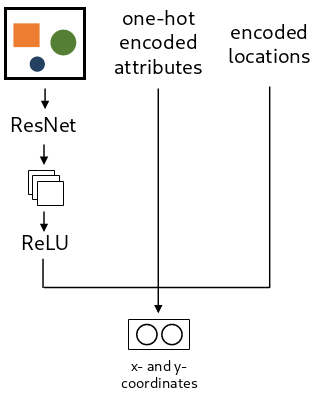
\includegraphics[width=0.35\linewidth]{figures/arch_coordinate_predictor.png}
        \label{fig:coordinate_predictor_architecture}
    }
    \subfigure[Model including incremental referring expression]{
        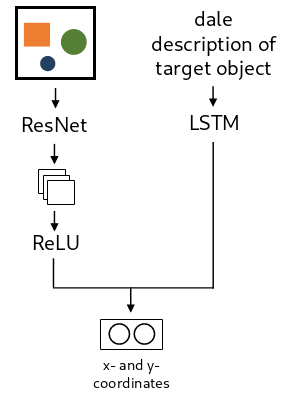
\includegraphics[width=0.34\linewidth]{figures/arch_coordinate_predictor_dale.png}
        \label{fig:coordinate_predictor_dale_architecture}
    }
    \caption{Simplified architectures of the \emph{coordinate reference resolvers}}
    % SD: How are these encoded?
    % DK: (done)
\end{figure}

In the first method, the target objects' attributes are encoded as \textbf{one-hot encodings}, as described in Section \ref{sec:object-identification}.
In an extension to this method, also the \textbf{center coordinates of all objects} in the image are included.
% SD: Encoded locations?
% DK: (done)
The center coordinates of all objects are simply extracted.
Since there is no direct way of ordering objects, distributed in 2 dimensions into a list, these are shuffled, to just provide the model with all possible targets to choose from.
Since there are varying numbers of objects in the image, this vector of variable length is padded to the maximum number of objects in the dataset.
The padded locations consist of two zeros for both coordinates.
In both methods, the encodings of the target object are concatenated with the encoded image and then passed to the coordinate predictor.
% SD: Why shuffled? If we order them the way they appear in the image, the model will have more information that they are sequentially related.
% DK: (done)
% SD: Convolutions are only applied on visual features, not object attribute features and locations.
% DK: (done)

The third method encodes the attributes of the target object with human language using the \textbf{incremental GRE-algorithm}.
This opposes the idea described before, to share as few natural language information as possible with the model.
Still, this approach can help to understand and analyze if the model was able to extract information about the objects and more specifically their attributes from the image.
% SD: The question you are asking is whether it is possible to predict location from the visual appearance of the object. This is highly complex task as it requires quite two step reasoning, identification of features with that attribute, e.g. blue and then locating that feature in the image.
% DK: TODO
If the model is able to match parts of the image with human words it would show that the model learned this attribute.
If the model in a next step can learn this for the whole dataset, this would mean that it could generalize over these attributes and assign them to certain regions in an image.
This insight would help for succeeding models that make use of these learnings without human language.

% Using the algorithm, one can describe an object using its attributes to discriminate it from other objects as efficiently as possible.
% In other words, the object is described unambiguously using the lowest number of words.
% The algorithm assumes that there is an order of importance for attributes, such as shape, color and size.
% This order defines, which attributes can be left out, while still identifying the object uniquely.
% This research relies on the following order from most important to least important: shape, color, size
% Given for example the scene from \ref{fig:clevr-dale-5} with the target object being the \emph{big purple cylinder}.
% Using all three attributes, this description identifies the object perfectly and uniquely.
% Following the algorithm, we could make the description shorter by removing the least important attribute \emph{size} without loosing unambiguity, describing it as the \emph{purple cylinder}.
% This can be taken even one step further by removing also the \emph{color}.
% Describing it as the \emph{cylinder} still doesn't describe any distractor, since the target object is the only cylinder in the scene.
% % SD: See my point earlier about the reversed algorithm between the two tasks 
% % DK: TODO

For the experiments, each image is captioned with a referring expression of the target object using the described algorithm.
To include it in the model, the referring expressions need to be padded to an equal length.
In this case they are padded to a length of 3, which is the maximum number of attributes that can be used.
For this, as standard practice in captioning tasks, the referring expressions are padded at the end with a specified padding token.

In the model, the referring expression is encoded, using the \emph{GRE parser} submodule.
Here, the learned embeddings of each token are parsed by the LSTM and its final hidden state is then used as a summary of the complete referring expression.
Tokens are embedded with embedding dimensions $LSTM_e$ and the output of the LSTM has the size if $LSTM_o$.
The vocabulary that is used for the descriptions is based on 14 symbols, including the padding token.
Both the processed image and the final hidden state of the LSTM are flattened and concatenated, which is then passed through the coordinate predictor.
% SD: \citep and \citet Use Name (year) when you are referring to particular person and (Name, year) when you are referring to a paper. Hence, in this case it would be the latter.
% DK: done

The fourth method, to encode the target object utilizes \textbf{masking} of the image.
% SD: Oh, before we talked about 3 methods
% DK: done
The image is masked in the same way as in Section \ref{sec:referring_expression_generation}.
While even the one-hot encodings contain human language knowledge by translating human referring descriptions into a vector, the masking method will only point the model towards the target object without giving more information.
It therefore can only rely on its own extracted visual features and the inherent human bias in the image when looking at masked images.
% SD: The information in the masked image is still not enough to identify the precise location, only the region. Hence, it corresponds on attention in the attention models. But those are generating labels and not predicting coordinated. The task is still challenging.
% DK: TODO
Both original and masked image are processed as described in \ref{sec:image-processing} and afterwards passed through the coordinate predictor.

For all setups, the same hyperparameters as in the previous experiments are used: a learning rate of $1\times10^{-4}$, a batch size of 32 samples and 30 epochs, \emph{Adam} \citep{Kingma2015} as optimizer.
8000 randomly selected samples are used for training, the remaining 2000 samples for testing.
The loss is calculated using cross entropy.
Table \ref{tab:variables-reference-resolution} shows the variables that are changed during the experiments for each of the models.

\begin{table}[ht]
    \centering
    \begin{tabular}{lcccc}
        \toprule
                                      & $e_i$                 & $c$               & $LSTM_e$  & $LSTM_o$      \\
                                      & $[50, 100, 300, 500]$ & $[512,1024,2048]$ & $[15,30]$ & $[1000,1500]$ \\\midrule
        coordinate reference resolver & \times                & \times            & -         & -             \\
        + one-hot                     & \times                & \times            & -         & -             \\
        + one-hot + locations         & \times                & \times            & -         & -             \\
        + incremental RE              & \times                & \times            & \times    & \times        \\
        + masking                     & \times                & \times            & -         & -             \\
        \bottomrule
    \end{tabular}
    \caption{Variables for each model where $e_i$ is the image embedding dimension, $c$ the dimensions of the coordinate predictor, $LSTM_e$ the embedding dimensions for tokens in the LSTM and $LSTM_o$ the output dimension of the LSTM}
    \label{tab:variables-reference-resolution}
\end{table}

The test dataset is again evaluated on the euclidean distance of the predicted coordinates to the ground truth coordinates.
This distance needs to be minimized.
The mean of all calculated distances is calculated across the whole epoch, which results in a mean distance score per epoch.
Since this score only takes the average of all predictions into account it doesn't show how every prediction fared individually.
If for instance the prediction of one object is getting more precise with growing number of epochs, but the precision of another object gets worse, the mean distance will stay the same.
% SD: Yes that’s correct but through several epochs we hope we will refine the distance and standard deviation of the error. It should level out. It is not a problem. What you do with a circle and accuracy is that you make the task easier as your pointer is now not pointing to a point but to a larger area.
% DK: TODO
It doesn't reflect this change.
For that reason, we also introduced an accuracy score.
For that we defined a fixed size circle with a radius of 20 pixels around the center of each object.
If the model's prediction lies in this circle, it will be counted as a correct prediction, if it lies outside, it is a false prediction.
These scores are averaged for the epoch and result in an accuracy score, where 100\% means that all predictions were very close to the center coordinates and 0\% means that no predictions were close to the center coordinates.
% SD: But here the score will face the same problem with steward deviation. Hence the only difference here is that pointing is less precise.
% DK: TODO
This of course doesn't give a perfect representation since the size of the objects varies, but it will still show, how precise each individual prediction is.
A high accuracy may indicate that the model could identify this specific object better.

In the second approach, the \textbf{attention reference resolver} predicts a region around the center of the target object.
For this, the image is divided into 14\times14 regions.
The target area is located around the center of the target object, consisting of 3\times3 regions.
Hereby, the center of the target object is located in the central region.
The model is then tasked to predict the matrix $A = (a_{ij})$, where:
\begin{align*}
    a_{ij} =
    \begin{cases}
        1, & \text{if region $i,j$ in target area} \\
        0, & \text{otherwise}
    \end{cases}
\end{align*}

To do this, the model combines a representation of the image and a representation of the target object.
More specifically, the image is encoded using the \emph{image encoder} submodule, omitting the last \emph{max pool} layer.
By this, the resulting matrix has 128\times14\times14 dimension, corresponding to the 14\time14 regions.
For the target object, the incremental RE is passed through an LSTM as described before.
Both encodings are passed through two linear layers separately to project them to the projection dimension $p$, followed by the $tanh$ function.



The reference resolution models are trained on the 'CLEVR single' as well as on both 'Dale' datasets.
The 'CLEVR single' dataset should test the model if it can actually learn locations of an object.
Since the model relies on the extracted features of ResNet, locational information of the objects in the image might not be present anymore.
This is due the fact that CNNs compress information of the image summarizing small regions (convolutions) several times.
While this extracts the key features of objects in an image and might capture relational position between these objects, absolute locations might get lost as shown by \citet{Kelleher2017}.
% SD: Explain. w3 had a paper with John Kelleher on what spatial information is encoded in CNNs
% DK: (done)
Training on this dataset should make sure that the model can converge towards the correct pixels, utilizing these features.
In a next step, the 'Dale' datasets provide the actual problem of discriminating objects from each other and afterwards pointing to the correct one.
Here, the models should make use of the additional given referring expressions about the scene, as one-hot encodings of the attributes, descriptions using the incremental GRE-algorithm or the encoded locations.
'Dale-2' and 'Dale-5' provide two different difficulties for the model, where it needs to discriminate a target object from one or four distractors and then point towards it.
% SD: Point at not just discriminate
% DK: (done)
Latter task is assumed to be significantly harder.

\subsubsection*{Results}
Tables \ref{tab:results:reference-resolver} to \ref{tab:results:reference-resolver-masked} show the results of the five adaptions of the reference resolver.
Across the first three models (basic reference resolver, +one-hot, +one-hot+locations), the same patterns can be seen.

The \textbf{basic reference resolver} acts as a baseline for the other models.
Since this model doesn't have any information about the target object, it shouldn't be able to point towards the correct target object.
However, this model should learn underlying structures in the images that it can use to make better predictions.
Indeed, the model converges on all datasets to a certain limit.
Random guesses of the coordinates correspond to a mean distance of 95 pixels, given the image size of 224\times224 pixels, which the model can beat for all datasets.

\begin{table}[ht]
    \centering
    \begin{tabular}{cc|cc|cc|cc|cc}
        \toprule
              &        & \multicolumn{2}{c}{\textbf{CLEVR single}} & \multicolumn{2}{c}{\textbf{Dale-2}} & \multicolumn{2}{c}{\textbf{Dale-5}} & \multicolumn{2}{c}{\textbf{CLEVR color}}                                                                 \\  \cmidrule(lr){3-4}\cmidrule(lr){5-6}\cmidrule(lr){7-8}\cmidrule(lr){9-10}
        $e_i$ & $c$    & \textbf{loss}                             & \textbf{Acc.}                       & \textbf{loss}                       & \textbf{Acc.}                            & \textbf{loss} & \textbf{Acc.} & \textbf{loss} & \textbf{Acc.} \\\midrule
        {100} & {512}  & {2,45}                                    & {96\%}                              & {38,16}                             & {35\%}                                   & {46,44}       & {18\%}        & {51,8}        & {12\%}        \\
        {100} & {1024} & {2,18}                                    & {94\%}                              & {37,23}                             & {38\%}                                   & {47,38}       & {18\%}        & {52,04}       & {13\%}        \\
        {100} & {2048} & {3,44}                                    & {99\%}                              & {36,8}                              & {40\%}                                   & {46,77}       & {18\%}        & {51,29}       & {13\%}        \\
        {500} & {512}  & {2,71}                                    & {96\%}                              & {37,1}                              & {37\%}                                   & {47,28}       & {18\%}        & {51,01}       & {14\%}        \\
        {500} & {1024} & {2,61}                                    & {97\%}                              & {36,2}                              & {39\%}                                   & {48,6}        & {17\%}        & {52,73}       & {12\%}        \\
        {500} & {2048} & {5,18}                                    & {99\%}                              & {36,09}                             & {40\%}                                   & {44,81}       & {18\%}        & {51,8}        & {13\%}        \\
        \bottomrule
    \end{tabular}
    \caption{Mean loss and accuracy of the basic reference resolver for different configurations of the model after 40 epochs: $e_i$ is the image embedding dimension and $c$ the coordinate predictor dimension}
    \label{tab:results:reference-resolver}
\end{table}

\begin{table}[b]
    \centering
    \begin{tabular}{cc|cc|cc|cc|cc}
        \toprule
              &        & \multicolumn{2}{c}{\textbf{CLEVR single}} & \multicolumn{2}{c}{\textbf{Dale-2}} & \multicolumn{2}{c}{\textbf{Dale-5}} & \multicolumn{2}{c}{\textbf{CLEVR color}}                                                                 \\  \cmidrule(lr){3-4}\cmidrule(lr){5-6}\cmidrule(lr){7-8}\cmidrule(lr){9-10}
        $e_i$ & $c$    & \textbf{loss}                             & \textbf{Acc.}                       & \textbf{loss}                       & \textbf{Acc.}                            & \textbf{loss} & \textbf{Acc.} & \textbf{loss} & \textbf{Acc.} \\\midrule
        {100} & {512}  & {2,95}                                    & {98\%}                              & {37,27}                             & {34\%}                                   & {47,05}       & {18\%}        & {51,25}       & {12\%}        \\
        {100} & {1024} & {3,64}                                    & {98\%}                              & {37,19}                             & {37\%}                                   & {46,39}       & {19\%}        & {50,25}       & {14\%}        \\
        {100} & {2048} & {6,15}                                    & {99\%}                              & {37,04}                             & {39\%}                                   & {45,77}       & {18\%}        & {50,55}       & {14\%}        \\
        {500} & {512}  & {3,29}                                    & {98\%}                              & {38,58}                             & {34\%}                                   & {47,25}       & {18\%}        & {50,56}       & {14\%}        \\
        {500} & {1024} & {2,15}                                    & {93\%}                              & {37,18}                             & {40\%}                                   & {47,57}       & {18\%}        & {51,75}       & {14\%}        \\
        {500} & {2048} & {2,86}                                    & {98\%}                              & {35,71}                             & {41\%}                                   & {46,62}       & {18\%}        & {52,67}       & {11\%}        \\
        \bottomrule
    \end{tabular}
    \caption{Mean loss and accuracy of the \emph{reference resolver + one-hot} for different configurations of the model after 40 epochs: $e_i$ is the image embedding dimension and $c$ the coordinate predictor dimension}
    \label{tab:results:reference-resolver-one-hot}
\end{table}

\begin{table}[ht]
    \centering
    \begin{tabular}{cc|cc|cc|cc|cc}
        \toprule
              &        & \multicolumn{2}{c}{\textbf{CLEVR single}} & \multicolumn{2}{c}{\textbf{Dale-2}} & \multicolumn{2}{c}{\textbf{Dale-5}} & \multicolumn{2}{c}{\textbf{CLEVR color}}                                                                 \\  \cmidrule(lr){3-4}\cmidrule(lr){5-6}\cmidrule(lr){7-8}\cmidrule(lr){9-10}
        $e_i$ & $c$    & \textbf{loss}                             & \textbf{Acc.}                       & \textbf{loss}                       & \textbf{Acc.}                            & \textbf{loss} & \textbf{Acc.} & \textbf{loss} & \textbf{Acc.} \\\midrule
        {100} & {512}  & {3,02}                                    & {97\%}                              & {36,88}                             & {37\%}                                   & {47,04}       & {16\%}        & {51,36}       & {12\%}        \\
        {100} & {1024} & {2,48}                                    & {95\%}                              & {38,24}                             & {33\%}                                   & {46,91}       & {15\%}        & {52,67}       & {12\%}        \\
        {100} & {2048} & {3,8}                                     & {100\%}                             & {37,89}                             & {32\%}                                   & {45,33}       & {13\%}        & {49,12}       & {11\%}        \\
        {500} & {512}  & {3,6}                                     & {98\%}                              & {35,56}                             & {42\%}                                   & {47,41}       & {16\%}        & {51,86}       & {12\%}        \\
        {500} & {1024} & {2,51}                                    & {98\%}                              & {36,56}                             & {39\%}                                   & {45,88}       & {17\%}        & {51,73}       & {12\%}        \\
        {500} & {2048} & {2,37}                                    & {97\%}                              & {37,33}                             & {35\%}                                   & {48,04}       & {16\%}        & {53,68}       & {11\%}        \\
        \bottomrule
    \end{tabular}
    \caption{Mean loss and accuracy of the \emph{reference resolver + one-hot + locations} for different configurations of the model after 40 epochs: $e_i$ is the image embedding dimension and $c$ the coordinate predictor dimension}
    \label{tab:results:reference-resolver-one-hot-location}
\end{table}

Table \ref{tab:results:reference-resolver} shows the results.
When trained on the 'CLEVR single' dataset, the model can minimize the mean loss consistently across all variations of the variables to a few pixels.
In effect, this means, that the model is able to almost always predict the correct location of the center of the target object.
Since no distractor is present, the model also doesn't need any description of the target object and only needs to discriminate the object from the background.
This shows that the model is in general able to derive geometrical information from abstract feature, extracted by a feature extractor.
Geometrical information therefore doesn't get completely lost during this abstraction, but the model is able to point to a specific object, as long as only one object is part of the image.
% SD: Because it is in the same location?
% DK: (done)

However, the model has more difficulties when distractors are present in the image.
For the 'Dale-2' dataset, the mean loss converges towards 35 to 39 pixels
The model was able to extract some structural information from the image, but the predictions are not consistently on the target object.
Looking at the accuracy, the best variations of the models are only able to point in 41\% to 42\% of the samples towards the correct object, which lies just below a random guess of 50\%.
Using the 'Dale-5' and the 'CLEVR color' datasets, the results are similar.
While the mean loss stays consistently around 46 to 48 pixels and 50 to 53 pixels respectively, they are still far below the random baseline.
Also the accuracies, lie a bit below the random guesses of 20\% and 15\% respectively.
However, it is visible that more present distractors in the scene challenge the model more.
% SD: What is the image size? What is the size of a typical object? 50 sounds quite good. Attention is predicting one of 7x7 blocks. Is 50 more or less than 1/7 of an image? 
% DK: (done)

Looking at the image embedding size $e_i$ and the coordinate predictor dimension $c$, it seems, they don't have any significant effect on the results.
The results staying the same across all variations indicates that the increase compared to the random baseline is just due to learning an underlying structural pattern of how scenes are set up.
This hypothesis will be discussed further below with examples from the predictions.

Interestingly, providing the model with the target object encoded as a \textbf{one-hot vector} and the \textbf{locations} of all objects doesn't improve the results.
% SD: Perhaps arranging the objects sequentially would help the model learn spatial contiguity, see my earlier comment.
% DK: TODO
Tables \ref{tab:results:reference-resolver-one-hot} and \ref{tab:results:reference-resolver-one-hot-location} show the same results as for the \emph{basic reference resolver}.
It seems that the model is not able to combine the image representation with the representation of that target object or the locations of all objects and another representation is needed.

\begin{table}[hb]
    \centering
    \begin{tabular}{cccc|cc|cc|cc}
        \toprule
              &        &          &          & \multicolumn{2}{c}{\textbf{Dale-2}} & \multicolumn{2}{c}{\textbf{Dale-5}} & \multicolumn{2}{c}{\textbf{CLEVR color}}                                                 \\  \cmidrule(lr){5-6}\cmidrule(lr){7-8}\cmidrule(lr){9-10}
        $e_i$ & $c$    & $LSTM_o$ & $LSTM_e$ & \textbf{loss}                       & \textbf{Acc.}                       & \textbf{loss}                            & \textbf{Acc.} & \textbf{loss} & \textbf{Acc.} \\\midrule
        {50}  & {1024} & {1000}   & {15}     & {22,64}                             & {63,55\%}                           & {48,23}                                  & {14,95\%}     & {52,62}       & {11\%}        \\
        {50}  & {2048} & {1500}   & {15}     & {21,35}                             & {65,9\%}                            & {46,95}                                  & {16,75\%}     & {52,2}        & {11,35\%}     \\
        {100} & {1024} & {1000}   & {15}     & \textbf{16,08}                      & \textbf{75,5\%}                     & {47,62}                                  & {16,5\%}      & {50,65}       & {12,8\%}      \\
        {100} & {1024} & {1000}   & {30}     & {20,69}                             & {69,5\%}                            & {46,9}                                   & {16,45\%}     & {51,23}       & {12,2\%}      \\
        {100} & {1024} & {1500}   & {15}     & {21,24}                             & {66,3\%}                            & {48,78}                                  & {15,55\%}     & {52,21}       & {12,25\%}     \\
        {100} & {2048} & {1000}   & {15}     & {19,46}                             & {70,1\%}                            & {46,79}                                  & {16,9\%}      & {50,24}       & {13,3\%}      \\
        {100} & {2048} & {1500}   & {15}     & {21,19}                             & {66,65\%}                           & {46,79}                                  & {16,65\%}     & {50,55}       & {11,3\%}      \\
        {300} & {1024} & {1000}   & {15}     & {20,63}                             & {68\%}                              & {46,91}                                  & {17,4\%}      & {50,39}       & {11,75\%}     \\
        {300} & {1024} & {1500}   & {15}     & {21,38}                             & {66,15\%}                           & {46,36}                                  & {15,55\%}     & {51,29}       & {12,25\%}     \\
        {300} & {2048} & {1000}   & {15}     & {21,12}                             & {66,95\%}                           & {46,98}                                  & {16,65\%}     & {51,4}        & {12,85\%}     \\
        {300} & {2048} & {1500}   & {15}     & \textbf{14,01}                      & \textbf{79,45\%}                    & {47,41}                                  & {16,9\%}      & {51,32}       & {12,6\%}      \\
        {300} & {2048} & {1500}   & {30}     & {22,09}                             & {64,75\%}                           & {46,77}                                  & {17,65\%}     & {49,75}       & {13,4\%}      \\
        {500} & {1024} & {1000}   & {15}     & {35,14}                             & {41,25\%}                           & {46,41}                                  & {16,6\%}      & {50,63}       & {12,8\%}      \\
        {500} & {2048} & {1500}   & {15}     & {36,52}                             & {41,95\%}                           & {44,9}                                   & {18,65\%}     & {50,02}       & {13,4\%}      \\
        \bottomrule
    \end{tabular}
    \caption{Mean loss and accuracy of the \emph{reference resolver + incremental RE} for different configurations of the model after 40 epochs: $e_i$ is the image embedding dimension, $c$ the coordinate predictor dimension, $LSTM_o$ the output dimension of the LSTM and $LSTM_e$ the embedding dimensions for tokens in the LSTM}
    \label{tab:results:reference-resolver-gre}
\end{table}

Encoding the attributes of the target object with the \textbf{incremental GRE-algorithm} finally improves the model's performance.
Table \ref{tab:results:reference-resolver-gre} shows the results of selected configurations.
Using the 'Dale-2' dataset, the model is able to predict the center coordinates of the target object for most of the images.
The results, hereby, are dependent on the different variables.
The best results are achieved with $e_i=300$, $c=2048$, $LSTM_o=1500$ and $LSTM_e=15$ and this configuration will be used in the succeeding analysis and the remaining language games experiments.
With this configuration the mean distance of the model's predictions is around 14 pixels, and they lie in around 79,45\% of the cases on the target object.
This is far below the random guess of the center coordinates as well as better than a random choice between the objects.
Comparing it to the other configurations, it becomes apparent that an image embedding size $e_i$ between 100 and 300 dimensions provides the model with enough information from the image.
Contrary to this, a relatively high decoder size of the LSTM $LSTM_o$ that decodes the referring expression is necessary.
However, it seems to be dependent on $e_i$.
A larger $e_i$ requires a larger $LSTM_o$.
Preliminary experiments have shown that lower sizes didn't provide any good results.
Furthermore, lower embedding dimensions of the tokens $LSTM_e$ tend to give better results.
An $LSTM_e$ around the vocabulary size of 14 gave the best results while for instance more dimensions with 30 always worsened the model.

Using the 'Dale-5' and 'CLEVR color' datasets, providing the incremental referring expression to the model didn't help.
The results are similar to the baseline with no information about the target object.

Finally, Table \ref{tab:results:reference-resolver-masked} shows the results, when the model is additionally provided with the \textbf{masked image}.
Hereby, the model is able to predict correct locations using all datasets.
All configurations achieve mean distances of a few pixels and accuracies of almost 100\%.
This shows that the model can make use of the masked image.
However, this is also not surprising since the model doesn't need to use the original image, but can completely rely on the mask.
Since the mask only includes the target object but no distractors, it corresponds to the 'CLEVR single' dataset which as already seen in the results before is an easy task to learn for the model.

\begin{table}[ht]
    \centering
    \begin{tabular}{cc|cc|cc|cc}
        \toprule
              &        & \multicolumn{2}{c}{\textbf{Dale-2}} & \multicolumn{2}{c}{\textbf{Dale-5}} & \multicolumn{2}{c}{\textbf{CLEVR color}}                                                 \\  \cmidrule(lr){3-4}\cmidrule(lr){5-6}\cmidrule(lr){7-8}
        $e_i$ & $c$    & \textbf{loss}                       & \textbf{Acc.}                       & \textbf{loss}                            & \textbf{Acc.} & \textbf{loss} & \textbf{Acc.} \\\midrule
        {100} & {512}  & {8,01}                              & {98\%}                              & {6,77}                                   & {100\%}       & {6,05}        & {95\%}        \\
        {100} & {1024} & {8,77}                              & {99\%}                              & {3,61}                                   & {98\%}        & {5,29}        & {93\%}        \\
        {100} & {2048} & {8,71}                              & {99\%}                              & {4,28}                                   & {96\%}        & {3,24}        & {93\%}        \\
        {500} & {512}  & {14,27}                             & {99\%}                              & {9,97}                                   & {99\%}        & {5,9}         & {94\%}        \\
        {500} & {1024} & {8,6}                               & {99\%}                              & {2,07}                                   & {94\%}        & {13,03}       & {95\%}        \\
        {500} & {2048} & {2,67}                              & {95\%}                              & {10,57}                                  & {96\%}        & {4,24}        & {98\%}        \\
        \bottomrule
    \end{tabular}
    \caption{Mean loss and accuracy of the \emph{reference resolver + masking} for different configurations of the model after 40 epochs: $e_i$ is the image embedding dimension and $c$ the coordinate predictor dimension}
    \label{tab:results:reference-resolver-masked}
\end{table}

\begin{figure}[ht]
    \centering
    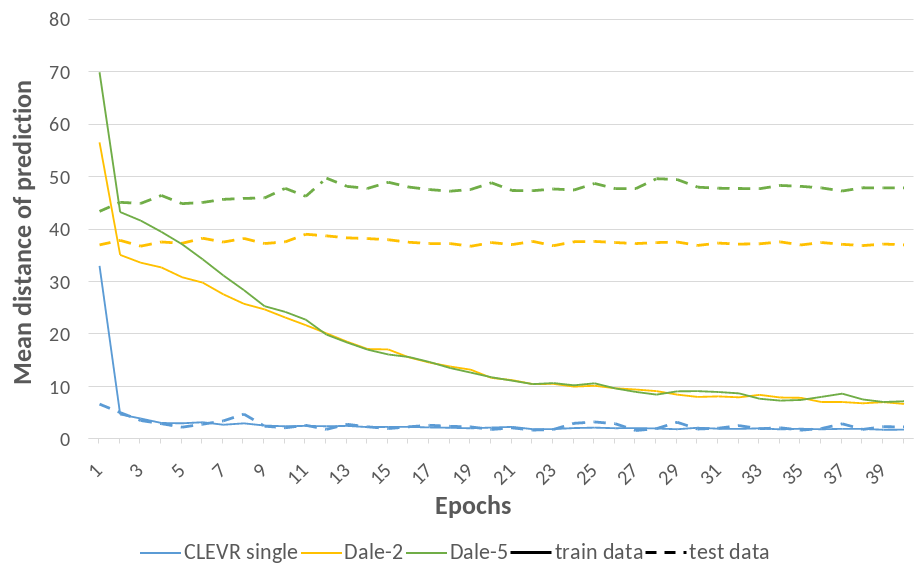
\includegraphics[width=0.8\linewidth]{figures/coordinate-predictor_loss.png}
    \caption{Mean loss of training and testing data with all datasets, using attributes encoded with the incremental GRE algorithm. The following variables are used for all models: $e_i=300$, $c=2048$, $LSTM_o=1500$, $LSTM_e=15$}
    \label{fig:coordinate-predictor_loss}
\end{figure}

Figure \ref{fig:coordinate-predictor_loss} gives more insight in why the models don't converge to a lower mean loss.
It shows how the mean loss changes during the training after each epoch.
Hereby, the figure shows the graph for the best performing configuration of the model that is presented with the incremental referring expression, using $e_i=300$, $c=2048$, $LSTM_o=1500$ and $LSTM_e=15$.
The different colors correspond to the different datasets.
Two lines are shown for each dataset.
The solid line represents the loss when trained on the training data.
The dotted line shows the mean distance to the target object of the model's predictions when presented with the unseen test data.
In particular, after each epoch, the model is frozen and tested on the test split.
After this, the weights are unfrozen again and the training is continued.
As can be seen, the training loss of the model always converges towards a low value.
Unsurprisingly, the datasets with fewer distractors are faster to learn than ones with more.
For both successful datasets, 'CLEVR single' and 'Dale-2', also the training loss converges towards the same value.
However, the testing curves for the remaining two datasets don't match their corresponding training curve.
Indeed, both curves stay at the same value until around epoch 9.
Then the loss of the training starts to drop while the loss in the testing starts to rise.
That indicates that until epoch 9, the model learns to general structural patterns in the images that apply to the complete dataset, both training and testing split.
After this, the model begins to memorize the training samples.
This knowledge is not transferrable to the test split and indeed even harms the test performance slightly.
That behavior can be observed for all models and configurations that don't outperform the baseline.
Preliminary experiments showed that applying dropout to help the model to generalize didn't increase the performance which shows that the architecture is not able to extract the necessary features from the images and the referring expression and combine them.
% SD: The results show that the model is learning something from the training data but this is not the feature that should be learning as the performance on the test data is low. Actually, is it low, it is 10, 35 and 45 pixels. We should not expect any difference between epochs as there is no training. Hence, a flat line is expected.
% DK: (done)

\begin{figure}[ht]
    \centering
    \subfigure['Dale-2', train split]{
        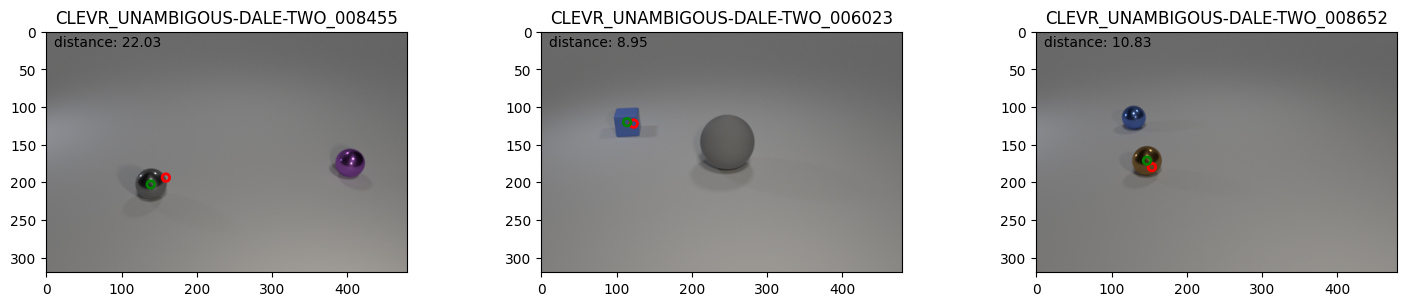
\includegraphics[width=.839\linewidth]{figures/visualization_dale-2_train.png}
        \label{fig:visualizations_dale-2_train}
    }
    \subfigure['Dale-2', test split]{
        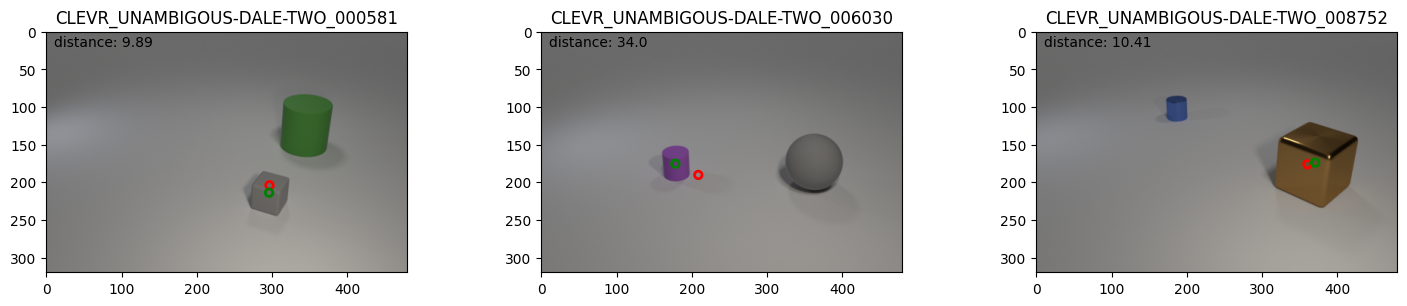
\includegraphics[width=.839\linewidth]{figures/visualization_dale-2_test.png}
        \label{fig:visualizations_dale-2_test}
    }
    \subfigure['Dale-5', train split]{
        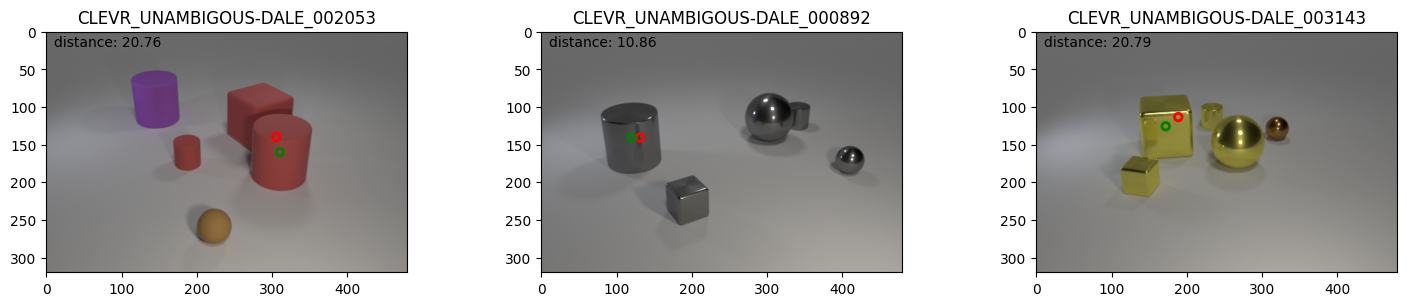
\includegraphics[width=.839\linewidth]{figures/visualization_dale-5_train.png}
        \label{fig:visualizations_dale-5_train}
    }
    \subfigure['Dale-5', test split]{
        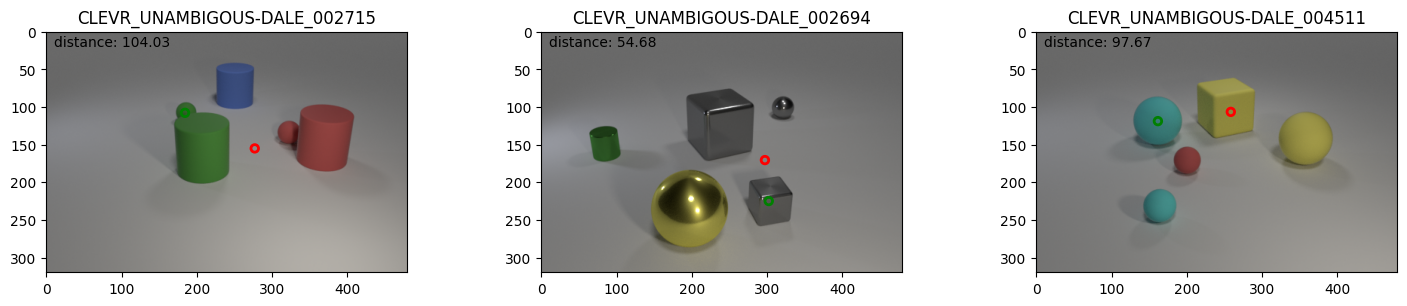
\includegraphics[width=.839\linewidth]{figures/visualization_dale-5_test.png}
        \label{fig:visualizations_dale-5_test}
    }
    \subfigure['CLEVR color', train split]{
        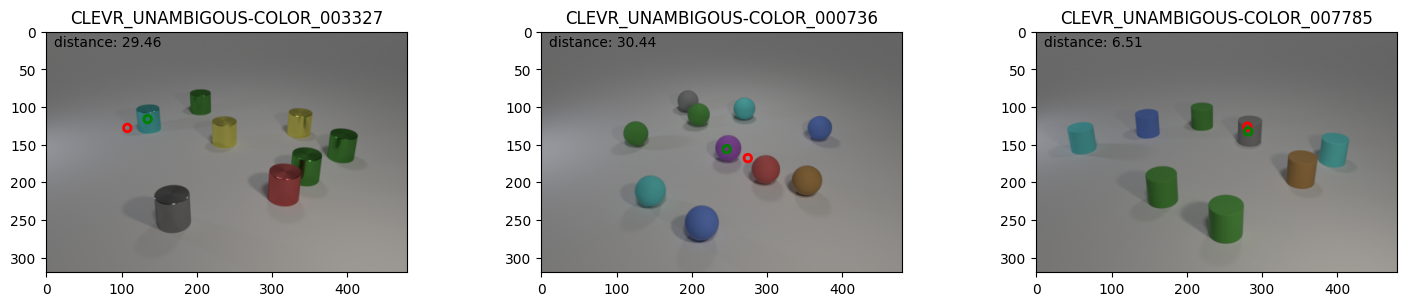
\includegraphics[width=.839\linewidth]{figures/visualization_colour_train.png}
        \label{fig:visualizations_colour_train}
    }
    \subfigure['CLEVR color', test split]{
        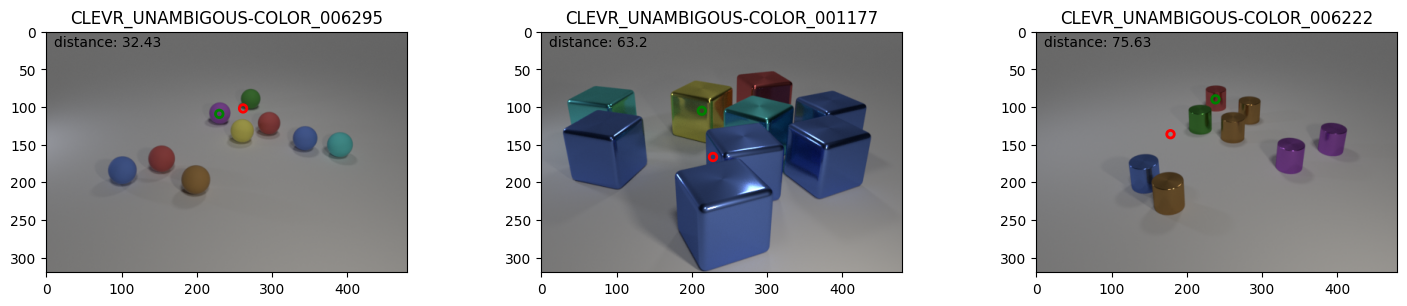
\includegraphics[width=.839\linewidth]{figures/visualization_colour_test.png}
        \label{fig:visualizations_colour_test}
    }
    \caption{Examples of the models' predictions on the 'Dale' and 'CLEVR color' datasets. The green circle represents the target object, the red object the model's prediction. Notice that the images are shown in the original size while the model processes them normalized. Hence, the distances don't correspond to the axes.}
    \label{fig:visualizations}
\end{figure}

An interesting pattern appears when doing a qualitative analysis of the models' predictions.
Here, the predicted coordinates compared to the ground truth coordinates are visualized (Figure \ref{fig:visualizations}), using the best performing model with $e_i=300$, $c=2048$, $LSTM_o=1500$ and $LSTM_e=15$.
Figure \ref{fig:visualizations_dale-2_train} shows random examples of predictions for images in the train dataset of Dale-2.
The green circle shows the ground truth center coordinates of the target object, while the red circle shows the prediction of the model.
As can be seen, the predictions are very precise.
Figure \ref{fig:visualizations_complete} combines the predictions and ground truths across all images in the train dataset.
This shows general patterns of the models predictions over the complete dataset.
Here, all predicted coordinates are placed as red circles into the image, while all ground truth coordinates are placed as green circles.
For the predictions on the 'Dale-2' dataset, the resulting shape is a rhombus, which reflects that all objects are placed usually central into the scene (see Figure \ref{fig:visualizations_dale-2_complete_train}).
As expected the green and red rhombus align mostly in the same area for the train split of the 'Dale-2' dataset.
% SD: But this image does not show clearly whether the circles for the same object match. You could calculate the average error in distance between the ground truth and predicted coordinates.
% DK: that is done in the quantitative analysis (mean square error above). The visualization should show general learned patterns of the model (as in this case predictions toard the center)
Figures \ref{fig:visualizations_dale-5_train} and \ref{fig:visualizations_dale-5_complete_train} show the same patterns for the 'Dale-5' dataset, while Figures \ref{fig:visualizations_colour_train} and \ref{fig:visualizations_colour_complete_train} show it for the 'CLEVR color' dataset.

The results look very different when using the predictions for the test split.
As discussed in the paragraphs above, the model performs well on the 'Dale-2' dataset which is also reflected in the qualitative analysis.
The visualization of the test split resembles the train split very much.
However, the other two datasets show differences.
As can be seen in Figures \ref{fig:visualizations_dale-5_test} and \ref{fig:visualizations_colour_test}, the three randomly selected predictions don't align with the ground truth coordinates.
While for some images they lie on a distractor, on some images, the prediction is on the background.
However, they tend to be in an area towards the target object, but are still quite imprecise.
% SD: They are closer to the target than distractor and you can see that it is working to a point. But remember this task is very challenging and I wouldn't say the results are so negative.
% DK: right, this is addressed in the conclusions below
These findings align with the mean distance scores, described in the paragraphs before.
However, it seems that the model's predictions are all towards the center of the image.
This can be seen clearer in Figures \ref{fig:visualizations_dale-5_complete_test} and \ref{fig:visualizations_colour_complete_test}.
Again, the green circles form the shape of rhombus.
In contrast, the predictions in red almost all cluster in the center of the image.
They form roughly the shape of a smaller rhombus.
% SD: There is a bias towards the centre but I would not say that the model has not learned anything. I'm surprised that it works so well given the feature representation we have, i.e. no geometric features.
% DK: again, conclusion below
% SD: The centre bias could be the way the error function is used, that is averages all distances and of course this has a tendency to some middle distance. A solution would be to have better geometric features that could take these errors better into account.
% DK: TODO (future work)

\begin{figure}[ht]
    \centering
    \subfigure['Dale-2', train split]{
        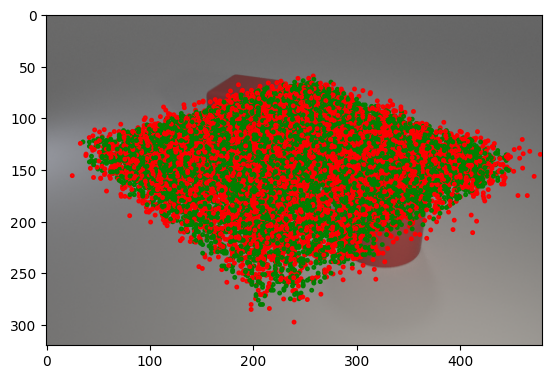
\includegraphics[width=0.42\linewidth]{figures/visualization_dale-2_train_complete.png}
        \label{fig:visualizations_dale-2_complete_train}
    }
    \subfigure['Dale-2', test split]{
        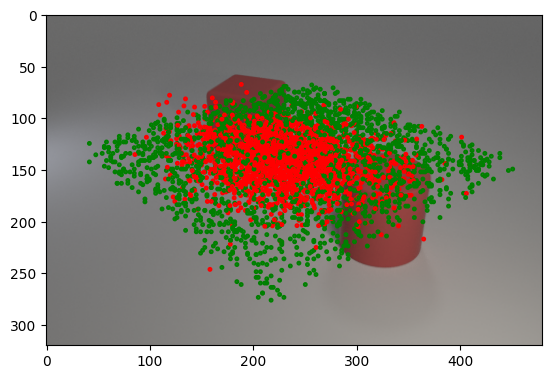
\includegraphics[width=0.42\linewidth]{figures/visualization_dale-2_test_complete.png}
        \label{fig:visualizations_dale-2_complete_test}
    }
    \subfigure['Dale-5', train split]{
        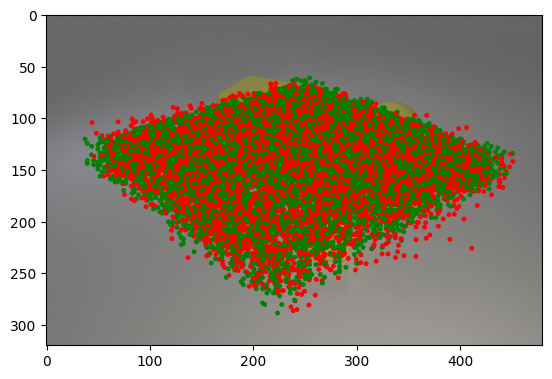
\includegraphics[width=0.42\linewidth]{figures/visualization_dale-5_train_complete.png}
        \label{fig:visualizations_dale-5_complete_train}
    }
    \subfigure['Dale-5', test split]{
        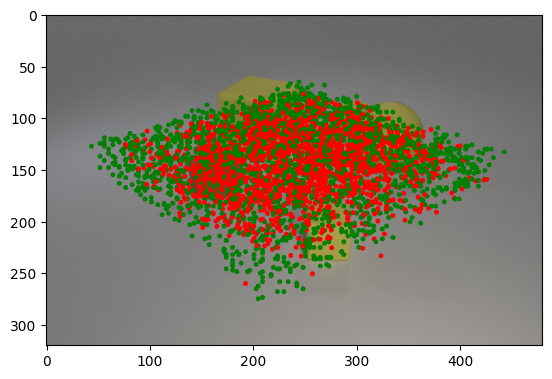
\includegraphics[width=0.42\linewidth]{figures/visualization_dale-5_test_complete.png}
        \label{fig:visualizations_dale-5_complete_test}
    }
    \subfigure['CLEVR color', train split]{
        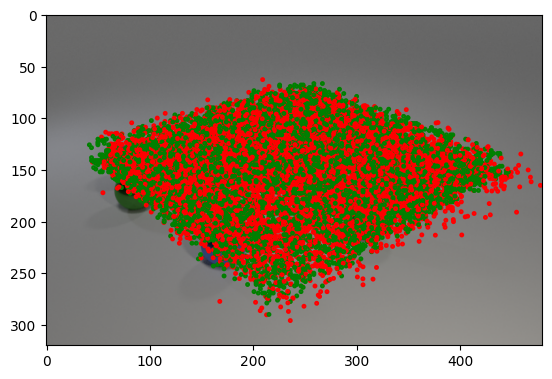
\includegraphics[width=0.42\linewidth]{figures/visualization_colour_train_complete.png}
        \label{fig:visualizations_colour_complete_train}
    }
    \subfigure['CLEVR color', test split]{
        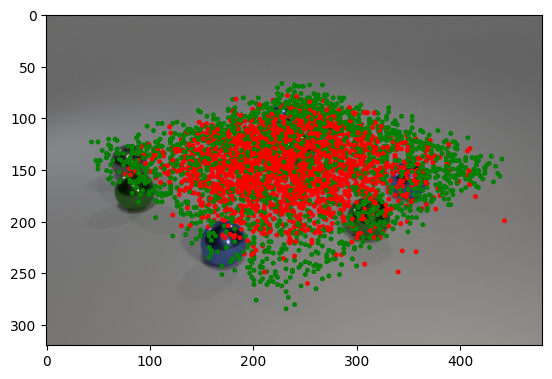
\includegraphics[width=0.42\linewidth]{figures/visualization_colour_test_complete.png}
        \label{fig:visualizations_colour_complete_test}
    }
    \caption{The images show all the model's predictions (red dots) and the ground truths (green dots) combined for the 'Dale' and 'CLEVR color' datasets}
    % SD: I Haven't checked the earlier captions, but the captions should be informative in the sense that one does not need to look for the text to understand them. Hence, include a brief summary of what each figure contains.
    % DK: (done)
    \label{fig:visualizations_complete}
\end{figure}

These results allow three conclusions.
First, the underlying structure in all images is the placement of objects in the center of the scene.
The models, learn to use the structure and are biased to predict coordinates towards the center.
% SD: centre - using British English?
% DK: so far I used always American English (hopefully consistently)
The reason for this is likely that the model can produce a relatively low loss, without relying on many extracted features of the objects.
Since all objects are always located in the center of the image and never in its corners, a prediction of any coordinate in the center is on average closer to the target object than any random prediction or predictions of coordinates at the borders of the image.
The model therefore learns only, where \emph{any} object is likely located and can minimize the mean distance to a certain extent with this strategy.

Secondly, even though the models are biased towards the center of the image, the predictions are still often leaning towards the location where many objects lie.
This can be seen for the 'CLEVR color' dataset, especially in left and central image in Figure \ref{fig:visualizations_colour_test}.
Again, by this strategy, the model can minimize the mean distance, since the probability is high that the target object lies in this cluster of objects.

Thirdly, when few distractors are present in the scene, the model is able to combine the encoding of the referring expression with the encoding of the image.
In particular, it is able to learn which of the objects in the image is described by the referring expression.
As soon as more objects are present, the task gets to difficult and the model only relies on the general patterns in the dataset.
Concluding, the model is able to extract, where objects are located in the image, but can't consistently make use of the referring expressions, to decide which of these objects is the target object.
% SD: There is a centre bias and the model can partially locate the target. The task is hard. The features are not optimal for this task. Future would should focus on using geometric features - we should have tried these and I'm sure we would get better results. Another extension would be making pointing less precise, i.e. focus on a single point, i.e. using a circle of 20 pixels or a 7x7 grid as in the attention mechanism. This would simplify the task.
% DK: TODO (future work)